\documentclass[11pt,a4paper]{article}

\usepackage[utf8]{inputenc} 
\usepackage[T1]{fontenc} 
\usepackage{lmodern}
\usepackage[margin=2cm]{geometry}
\usepackage[german]{babel}
\usepackage{array}
\setlength{\parindent}{0pt}
\setlength{\parskip}{1ex plus 0.5ex minus 0.5ex}

\usepackage{amsmath} 
\usepackage{graphicx} 
\usepackage{booktabs}
\usepackage[colorlinks]{hyperref}
\usepackage{nicefrac}
\usepackage{gensymb}
\usepackage[usenames,dvipsnames,svgnames,table]{xcolor}
\usepackage{multirow}
\usepackage{tikz}
%\usepackage{chemfig}

\hbadness=99999

\usepackage{etoolbox}

\makeatletter
\patchcmd{\@classz}
  {\CT@row@color}
  {\oldCT@column@color}
  {}
  {}
\patchcmd{\@classz}
  {\CT@column@color}
  {\CT@row@color}
  {}
  {}
\patchcmd{\@classz}
  {\oldCT@column@color}
  {\CT@column@color}
  {}
  {}
\makeatother

\begin{document}

{
\centering 
\large 
Physiklabor für Anf\"anger*innen \\
Ferienpraktikum im Sommersemester 2018 \\[4mm]
\textbf{\LARGE 
Versuch 36: Adiabatenexponenten
} \\[3mm]
(durchgef\"uhrt am 14.09.2018 bei Nico Strauß) \\
Andréz Gockel, Patrick M\"unnich, (Gruppe 14)\\
\today \\[10mm]
}

\tableofcontents
\pagebreak


\section{Ziel des Versuchs}

Das Ziel dieses Versuchs ist es den Adiabatenexponenten von Luft und Argon zu bestimmen \footnote{Kohlenstoffdioxid war original teil des Experiments, wurde aber ausgelassen da nicht genügend Druck vorhanden war, um eine Schwingung zu erzeugen.}. Zuerst bestimmen wir aus den Strukturformeln von Stickstoff und Argon deren Molekularen freiheitsgraden. Welche verwendet werden um den theoretischen Wert des Adiabatenexponentes herzuleiten. Um den Wert experimentell zu bestimmen wird ein Versuchsaufbau nach Rüchardt-Flammerfeld \ref{JS1} verwendet, womit die Schwingungsdauer des Schwingkörpers gemißt wird. Leitet man die Formel \ref{F:0} her, die den Adiabatenexponent in Abhängigkeit der Schwingungsdauer bringt kann man den dessen Wert bestimmen.


\section{Theoretische Bestimmung des Adiabatenexponenten}

Die strukturformel für Stickstoff ist %\chemfig{\lewis{4, N}~\lewis{0, N}} 
und für Argon ist %\chemfig{\lewis{0246, Ar}} \ N$\equiv$N
Um den theoretischen Wert zu bestimmen verwenden wir diese Näherung für die freiheitsgraden: $f = 3N-b$ \cite{Anleitung} die bei diesen Gasen bei Raumtemperatur gilt. Wobei $N$ die Anzahl der Atome ist und $b$ die Anzahl der Bindungen.

Der Adiabatenexponent $\kappa$ ist definiert als $\kappa = \frac{c_p}{c_V}$, wobei $c_p$ die isobare Wärmekapazität ist und $c_V$ die isochore Wärmekapazität, welche durch Betrachtung der inneren Energie des gases verallgemeinert werden können womit wir $\kappa = \frac{f+2}{f}$ bekommen. Mit der Näherung haben wir $\kappa = \frac{3N-b+2}{3N-b}$ Für Stickstoff haben wir zwei Atome mit 3 Bindungen:
$$\kappa = \frac{6-3+2}{6-3} = \frac{5}{3}$$
und für Argon mit einem Atom und null Bindungen bekommen wir ebenfalls:
$$\kappa = \frac{3-0+2}{3-0} = \frac{5}{3}$$


\section{Experimentelle Bestimmung des Adiabatenexponenten}
\subsection{Aufbau}

\subsection{Theorie}

\subsection{Auswertung und Fehleranalyse}

\subsection{Teil A - Umwandlung von mechanischer Arbeit in Wärme }
$$
\begin{array}{lc}
	\multicolumn{1}{l}{\textrm{Zu Bestimmende Werte}} \\
	\toprule 
	\textrm{Luftdruck} & p_A \\
	\textrm{Masse Schwingkörper} & m_{p} \\
	\textrm{Durchmesser des Glasrohres} & d\\
	\textrm{Periode} & n \\
	\textrm{Temperatur} & T\\
	\bottomrule \\
	\multicolumn{2}{l}{\textrm{Bekannte Werte}} \\
	\toprule
	\textrm{Volumen des Glaskolbens} & V = (2225 \pm 5)\,\textrm{cm}^3\\
	\bottomrule 
\end{array}
$$

\begin{equation}\tag{F1}
	\kappa = \frac{4 \pi^2 mV}{A^2 p T^2_s}
	\label{F:0}
\end{equation}
\subsubsection{Durchf\"uhrung}

\begin{figure}[h]
\centering
\fbox{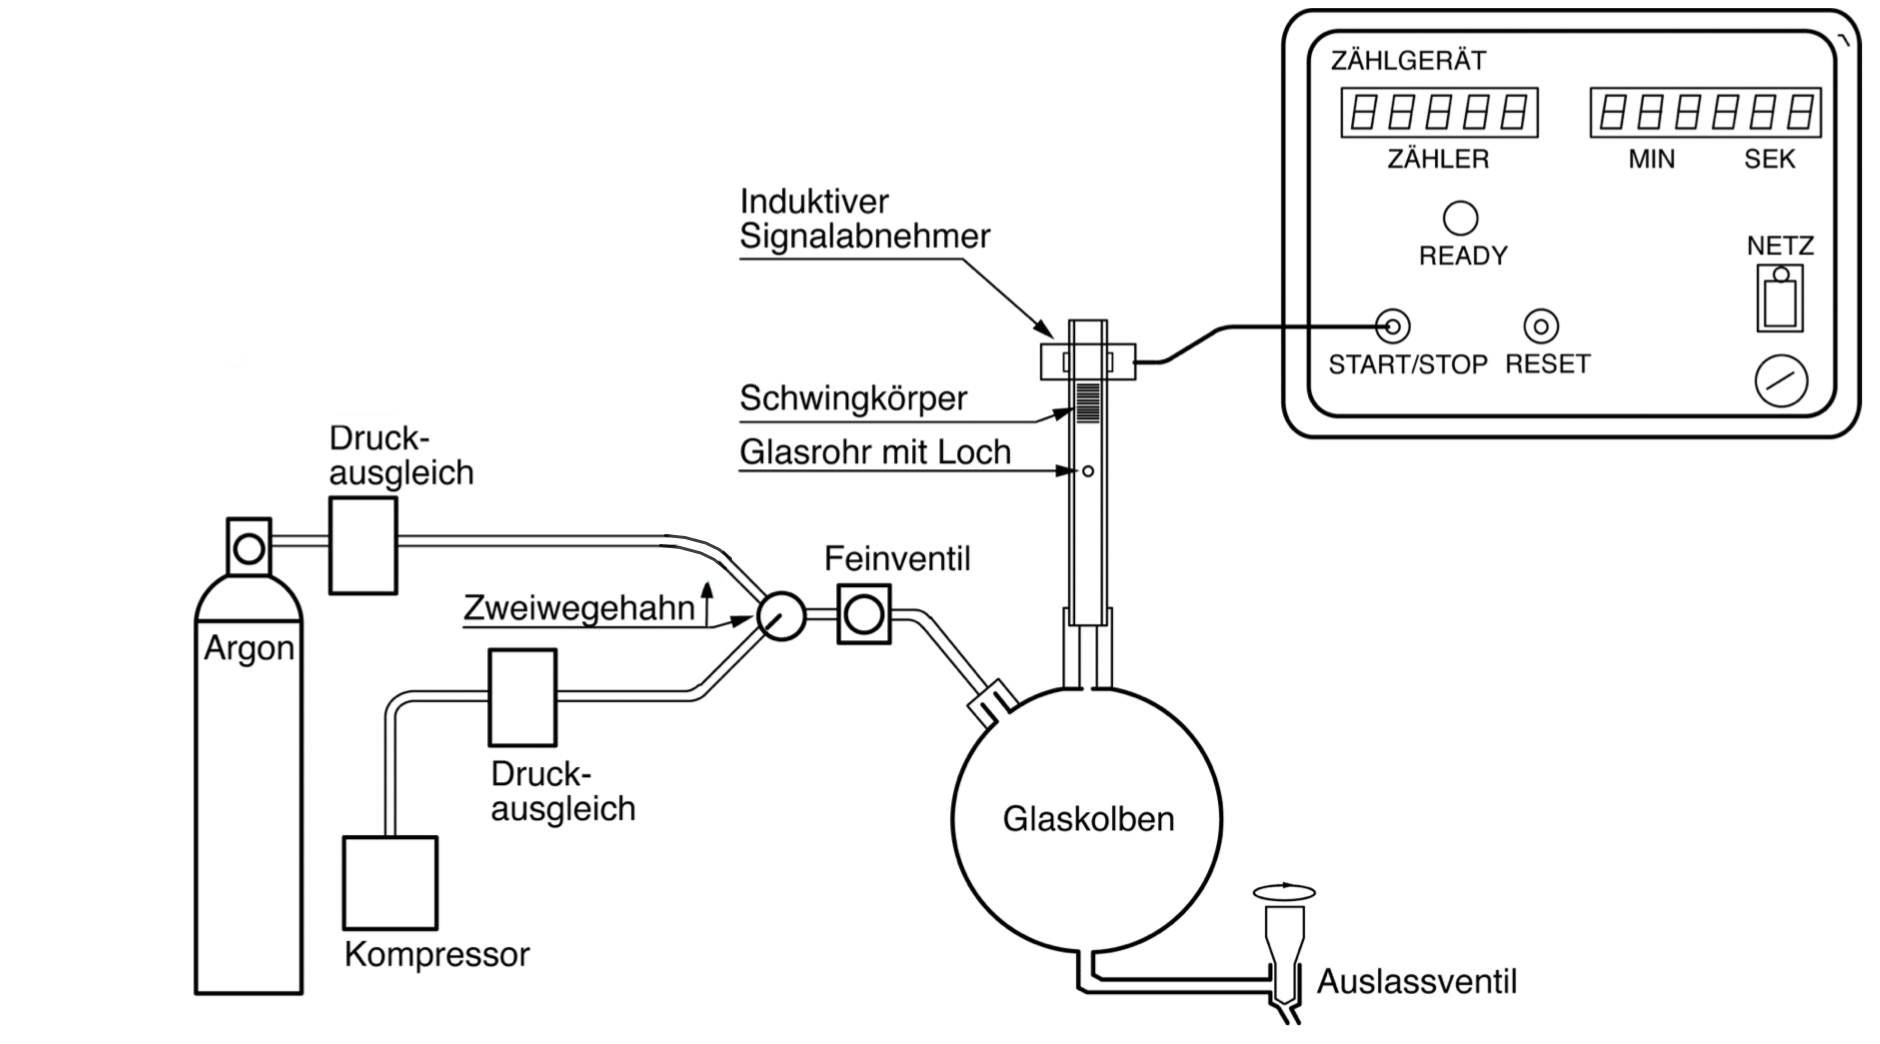
\includegraphics[width=0.8\textwidth]{auuufbauuu}}
   \renewcommand\thefigure{B1}
\caption{Versuchsaufbau}
\label{JS1}
\end{figure}


\subsubsection{Auswertung}

Die Messung wurde zweimal durchgef\"uhrt. Bei der ersten Durchf\"uhrung wurde die Temperatur\"anderung \"uber 50 Drehungen jeweils im Abstand von 10 Drehungen gemessen. Die zweite Durchf\"uhrung wurde mit 100 Drehungen durchgef\"uhrt und die Temperatur alle 5 Drehungen notiert. Die genauen Messwerte befinden sich im Anhang. \ref{table:m1}, \ref{table:m2}.

Die restlichen Messungen ergaben: $$m_W = 79.18(3)\,\textrm{g}, \quad m_{kal} = 98.05(3)\,\textrm{g}, \quad d = 4.765(3)\,\textrm{cm}$$

F\"ur die W\"armekapazit\"at gilt:\\

\begin{equation}
C=C_{Kal}+C_T+m_wc_w,\label{eq1}
\end{equation}

was umgestellt werden kann zu:

\begin{equation}
c_w=\frac{C-C_{Kal}-C_T}{m_w}.\label{eq2}
\end{equation}

$C$ wird hier mittels der folgenden Gleichungen bestimmt:

\begin{equation}
C=\frac{Q}{\Delta T}
\end{equation}

\begin{equation}
W_R=mgn\pi d=Q
\end{equation}

Mit unseren Messwerten und dem $uncertainties$ Paket \cite{Uncertainties} in Python berechnen wir damit:\\
$$\begin{tabular}{|c|c|c|c|c|}
\hline
\textrm{Messung} & 1 & 2 & \textrm{Mittelwert} & \textrm{Gewichtet} \\ 
\hline
\textrm{W\"armekapazit\"at} $\left[\mathrm{\nicefrac{\mathrm{J}}{kg K}}\right]$ & $8300\pm1400$ & $3500\pm600$ & $5900\pm800$ & $4187\pm 554$ \\
\hline
\end{tabular}$$

Diese Rechnungen wurden mit dem \textit{uncertainties} Paket in Python durchgef\"uhrt. Diese Rechnungen k\"onnen im Anhang gefunden werden..\\

Der Fehler der Messung mit dem Sch\"urholz Apparat ist aufgrund der gro\ss en Ungenauigkeit der Temperatur und der Anzahl Drehungen sehr gro\ss. Au\ss erdem ist es recht wahrscheinlich, dass $F_{R}$ und $F_{G}$ sich nicht st\"andig ganz ausgleichen, also dadurch auch eine Unsicherheit entsteht. Dies ist einflussreich, da die W\"arme, $Q$, von $F_R$ via $W_R=\int F_Rds$ abh\"angig ist. Da $F_R$ \"uber $F_G$ bestimmt wird und dies bei nicht korrekter Ausgleichung der Beiden nicht akkurat ist, ist also auch $Q$ und dadurch $c_w$ ungenau. Als systematischer Fehler kommt noch die Ungenauigkeit der Masse von 5\,kg hinzu. Der Literaturwert hierzu ist $4182$ $\mathrm{\nicefrac{\mathrm{J}}{kg K}}$. Der Unterschied beim normalen Mittelwert ist aufgrund der Messungenauigkeiten und niedrigen Anzahl Messungen sehr gro\ss.\\

Der gewichtete arithmetische Mittelwert ist jedoch sehr nahe an dem Literaturwert. Dies der Fall, da die zweite Messung wesentlich n\"aher dran ist und der Fehler dort wesentlich kleiner ist. Aufgrund der Formel f\"ur den gewichteten arithmetischn Mittelwert,

\begin{equation}
\overline{x}_g=\frac{\sum_ig_ix_i}{\sum_ig_i},
\end{equation}

mit den Gewichtsfaktoren

\begin{equation}
g_i=u_i^{-2},
\end{equation}

wird hier also der zweite Wert st\"arker gewichtet und wir bekommen einen Mittelwert, der um $t = 0.009$ vom Literaturwert abweicht. Dies wurde mit 

\begin{equation}
t=\frac{|x_0-y|}{u_x}\label{abw}
\end{equation}

berechnet.

\subsubsection{Diskussion}

\pagebreak

\subsection{Teil B - Umwandlung von elektrischer Arbeit in Wärme}

\subsubsection{Durchf\"uhrung}

\subsubsection{Auswertung}

Es wurden zwei Messungen durchgef\"uhrt mit jeweils $116.94\,$g und $113.42\,$g Wasser. Die Wassermenge wurde so gew\"ahlt, damit der Widerstand und das Thermometer in dem Wasser eingetaucht sind. Die Dauern der Messungen waren 38 und 20 Minuten. Diese wurden so gew\"ahlt, dass sie m\"oglichst kurz ausfallen sollten. Temperatur\"anderungen wurden im Abstand von 60 Sekunden gemessen, da diese sonst nicht auff\"allig genug w\"aren, um etwas zu erkennen. Die Messwerte hierzu sind aufgrund ihrer L\"ange im Anhang.

Das extrapolationsverfahren der 1. Messreihe ergibt $T_{max} = 26.5\celsius$ da der Temperaturabfall erst nach 30 begann. Für die 2. Messreihe ergibt das extrapolationsverfahren $T_{max} = 41.45\celsius$ \ref{Dia:1}, \ref{Dia:2}, \ref{Ext}

\begin{table}[h!]
	\centering
	\rowcolors{2}{gray!10}{white}
	\begin{tabular}{|c|cccc|}
		\multicolumn{5}{c}{\textrm{Extrapolationverfahren}} \\
		\noalign{\global\arrayrulewidth=0.4mm}
		\hline
		\noalign{\global\arrayrulewidth=0.2mm}
		\textrm{Messreihe} & $a$ in \celsius & $u_a$ in \celsius & b in $\nicefrac{\celsius}{\textrm{s}}$ & $u_b$ in $\nicefrac{\celsius}{\textrm{s}}$ \\
		\hline
	1 & 26.5 & 0.037 &  -33.579 & 2.105 $\times 10^{-5}$ \\
	2 & 42.65 & 1.605 & -0.0025 & 0.001443 \\
		\hline
	\end{tabular}
	\renewcommand\thetable{T3}
	\caption{Wertetabelle für die extrapolation}
	\label{Ext}
\end{table}

Uns ist bekannt, dass $W_{el}$ vollst\"andig in W\"armeenergie, $Q$, umgewandelt wird. Folgende Formeln gelten:

\begin{equation}
Q=(C_{Kal}+m_wc_w)\Delta T\label{Q_el}
\end{equation}
\begin{equation}
W_{el}=\int P\mathrm{d}t=\int UI\mathrm{d}t.
\end{equation}

Da $P$ konstant ist, kann man hier einfach mit

\begin{equation}
W_{el}=UI\Delta t\label{W_el}
\end{equation}

rechnen. Bei unserer Messreihe waren die werte f\"ur $U$ und $I$ jeweils 14.9\,V und 1.5\,A.\\

Stellen wir (\ref{Q_el}) nach $c_w$ um und setzen (\ref{W_el}) ein, so bekommen wir als Formel:

\begin{equation}
c_w=\frac{UI\frac{\Delta t}{\Delta T}-C_{Kal}}{m_w}.
\end{equation}

Unser $m_w$, die Masse des Wassers, ist wie oben erw\"ahnt bei der ersten Messreiehe $116.94(3)\,$g und bei der zweiten $113.42(3)\,$g. Somit ergeben unsere Werte f\"ur $c_w$:

\begin{table}[h!]
	\centering
	\rowcolors{2}{gray!10}{white}
	\begin{tabular}{|c|cccc|}
		\noalign{\global\arrayrulewidth=0.4mm}
		\hline
		\noalign{\global\arrayrulewidth=0.2mm}
		\textrm{Messung} & $1$ & $2$  & Mittelwert & Gewichtet\\
		\hline
	\textrm{W\"armekapazit\"at} $\left[\mathrm{\nicefrac{\mathrm{J}}{kg K}}\right]$ & $7330\pm0.09$ & $8790\pm0.11$ & $8060\pm0.10$ & $7931\pm0.07$ \\		
	\hline
	\end{tabular}
	\renewcommand\thetable{T3}
	\caption{Wertetabelle W\"armekapazit\"at}
	\label{Ext}
\end{table}

Der gewichtete arithmetische Mittelwert wurde gleich wie beim ersten Teil berechnet. Mit der Formel f\"ur die Abweichung aus Teil A, (\ref{abw}), sind wir hier $t = 53543$ von dem Literaturwert entfernt.\\

Der gro\ss e Unterschied zwischen den Abweichungen liegt vermutlich dabei, dass beim zweiten Versuch man wesentlich ungenauer ablesen musste. Dieses Problem ist durch die kurze Erw\"armungsphase vergr\"o\ss ert wordene. H\"atte man zu einer h\"oheren Temperatur erw\"armt, so w\"urde es sich auch schneller abk\"uhlen und man k\"onnte einen gr\"o\ss eren Temperaturabstand als Indikator f\"ur das Senken der Temperatur w\"ahlen.\\

Au\ss erdem haben wir noch einen systematischen Fehler aufgrund des R\"uhrens des Wassers, was zur Mischung dient, aber wodurch kinetische Energie hinzugef\"ugt wird, welches das Wasser auch aufw\"armt. Dazu kann man noch erw\"ahnen, dass die Au\ss entemperatur steigt, wodurch das Wasser nicht immer gleich abk\"uhlt. Dies ist jedoch aufgrund der kurzen Dauer der Messung nicht sehr einflussreich.

\subsubsection{Diskussion}

\vfill

\begin{thebibliography}{9}
 \bibitem{Uncertainties}''Correlations between variables are automatically handled, which sets this module apart from many existing error propagation codes.'' - https://pythonhosted.org/uncertainties/
 \bibitem{Anleitung} Physikalisches Institut der Albert-Ludwigs-Universität Freiburg (Hrsg.) (08/2018): Versuchsanleitungen zum Physiklabor für Anfänger*innen, Teil 1, Ferienpraktikum im Sommersemester 2018.
 \end{thebibliography}
%Systematische und statistische Fehler.

\pagebreak


\section{Anhang}




\begin{table}[h]
	\centering
	\rowcolors{2}{gray!10}{white}
	\begin{tabular}{|r|l|}
		\multicolumn{2}{c}{\textrm{Messreihe 1}} \\
		\noalign{\global\arrayrulewidth=0.4mm}
		\hline
		\noalign{\global\arrayrulewidth=0.2mm}
		\textrm{Rotationen }$n \pm 0.3$ & \textrm{Temperatur }$T \pm 0.05\celsius$\\
		\hline
		0 & 24 \\
		10 & 24.1 \\
		20 & 24.3 \\
		30 & 24.5 \\
		40 & 24.6 \\
		50 & 24.8 \\
		\hline
	\end{tabular}
	\renewcommand\thetable{T1}
	\caption{Messreihe 1 für Teil A}
	\label{table:m1}
\end{table}

\begin{table}[h]
	\centering
	\rowcolors{2}{gray!10}{white}
	\begin{tabular}{|r|l|}
		\multicolumn{2}{c}{\textrm{Messreihe 2}} \\
		\noalign{\global\arrayrulewidth=0.4mm}
		\hline
		\noalign{\global\arrayrulewidth=0.2mm}
		\textrm{Rotationen }$n \pm 0.3$ & \textrm{Temperatur }$T \pm 0.05\celsius$\\
		\hline
		0 & 24.3 \\
		5 & 24.3 \\
		10 & 24.4 \\
		15 & 24.5 \\
		20 & 24.6 \\
		25 & 24.7 \\
		30 & 24.8 \\
		35 & 24.9 \\
		40 & 25 \\
		45 & 25.1 \\
		50 & 25.2 \\
		55 & 25.2 \\
		60 & 25.4 \\
		65 & 25.5 \\
		70 & 25.5 \\
		75 & 25.6 \\
		80 & 25.6 \\
		85 & 25.7 \\
		90 & 25.8 \\
		95 & 26 \\
		100 & 26 \\
		\hline
	\end{tabular}
	\renewcommand\thetable{T2}
	\caption{Messreihe 2 für Teil A}
	\label{table:m2}
\end{table}

\begin{table}[h]
\centering
\rowcolors{2}{gray!10}{white}
\begin{tabular}{|>{\columncolor[gray]{1}}c|r|r|r|}
\multicolumn{2}{c}{}&\multicolumn{1}{c}{Luft} & \multicolumn{1}{c}{Argon}\\
\hline
Messreihe & Periode & Zeit in $s$ & Zeit in $s$\\
\hline 
&200$\pm14$  & 78.53  &  75.06 \\
&400$\pm20$  & 156.89 & 149.50 \\
&600$\pm25$  & 235.78 & 223.57 \\
&800$\pm28$  & 314.35 & 297.25 \\
\multirow{-5}{*}{1}
&1000$\pm32$ & 392.34 & 370.68 \\ 
\hline
&200$\pm14$  & 78.44  &  73.03 \\
&400$\pm20$  & 156.87 & 145.91 \\
&600$\pm25$  & 235.38 & 218.79 \\
&800$\pm28$  & 313.95 & 291.47 \\
\multirow{-5}{*}{2}
&1000$\pm32$ & 392.52 & 364.06 \\ 
\hline
&100$\pm10$ & 39.09 & 36.10 \\
&100$\pm10$ & 38.96 & 36.18 \\
&100$\pm10$ & 39.16 & 36.14 \\
&100$\pm10$ & 39.00 & 36.10 \\
\multirow{-5}{*}{3}
&100$\pm10$ & 39.96 & 36.16 \\ 
\hline
\end{tabular}
\renewcommand\thetable{T1}
\caption{1. Messwerte}
\label{tab:B1}
\end{table}

\begin{table}[h]
\centering
$\begin{array}{rl}
\multicolumn{2}{l}{\textrm{\underline{Unsicherheiten:}}}\\
\textrm{Zeit: } & \pm 0.03 \textrm{s}\\
\textrm{Temperatur: } & \pm 0.02 \textrm{\celsius}\\
\textrm{Strom: } & \pm 0.018 \textrm{A}\\
\textrm{Spannung: } & \pm 0.12 \textrm{V}
\end{array}$
\rowcolors{2}{gray!10}{white}
\begin{tabular}{|c|c|c|c|}
\multicolumn{4}{l}{Wasser 113.42(3)\,g}\\
\hline
$t$ in s & $T$ in $^\circ\textrm{C}$ & $I$ in A & $U$ in V \\
\hline 
0   & 22 & 1.5 & 14.9\\
60  & 22 & 1.5 & 14.9\\
120 & 23 & 1.5 & 14.9\\
180 & 24 & 1.5 & 14.9\\
240 & 26 & 1.5 & 14.9\\ 
300 & 27 & 1.5 & 14.9\\ 
360 & 28 & 1.5 & 14.9\\ 
420 & 29.2 & 1.5 & 14.9\\ 
480 & 30.3 & 1.5 & 14.9\\ 
540 & 31.9 & 1.5 & 14.9\\ 
600 & 33 & 1.5 & 14.9\\ 
660 & 33.7 & 1.5 & 14.9\\ 
720 & 35 & 1.5 & 14.9\\ 
780 & 35 & 1.5 & 14.9\\ 
840 & 36 & 1.5 &14.9\\
900 & 37 & 1.5 & 14.9\\
960 & 38.2 & 0 & 0\\
1020 & 39.5 & 0 & 0\\
1080 & 40 & 0 & 0\\
1140 & 40 & 0 & 0\\
1200 & 39.5 & 0 & 0\\
\hline
\end{tabular}
\phantom{$\begin{array}{rl}
\multicolumn{2}{l}{\textrm{\underline{Unsicherheiten:}}}\\
\textrm{Zeit: } & \pm 0.03 \textrm{s}\\
\textrm{Temperatur: } & \pm 0.02 \textrm{\celsius}\\
\textrm{Strom: } & \pm 0.018 \textrm{A}\\
\textrm{Spannung: } & \pm 0.12 \textrm{V}
\end{array}$
}
\renewcommand\thetable{T5}
\caption{2. Messwerte für Teil B}
\label{tab:B2}
\end{table}

\pagebreak

\pagebreak
\phantom{lol}
\end{document}